\chapter{Background Appendix}
% \begin{figure}[ht!]
%     \centering
%     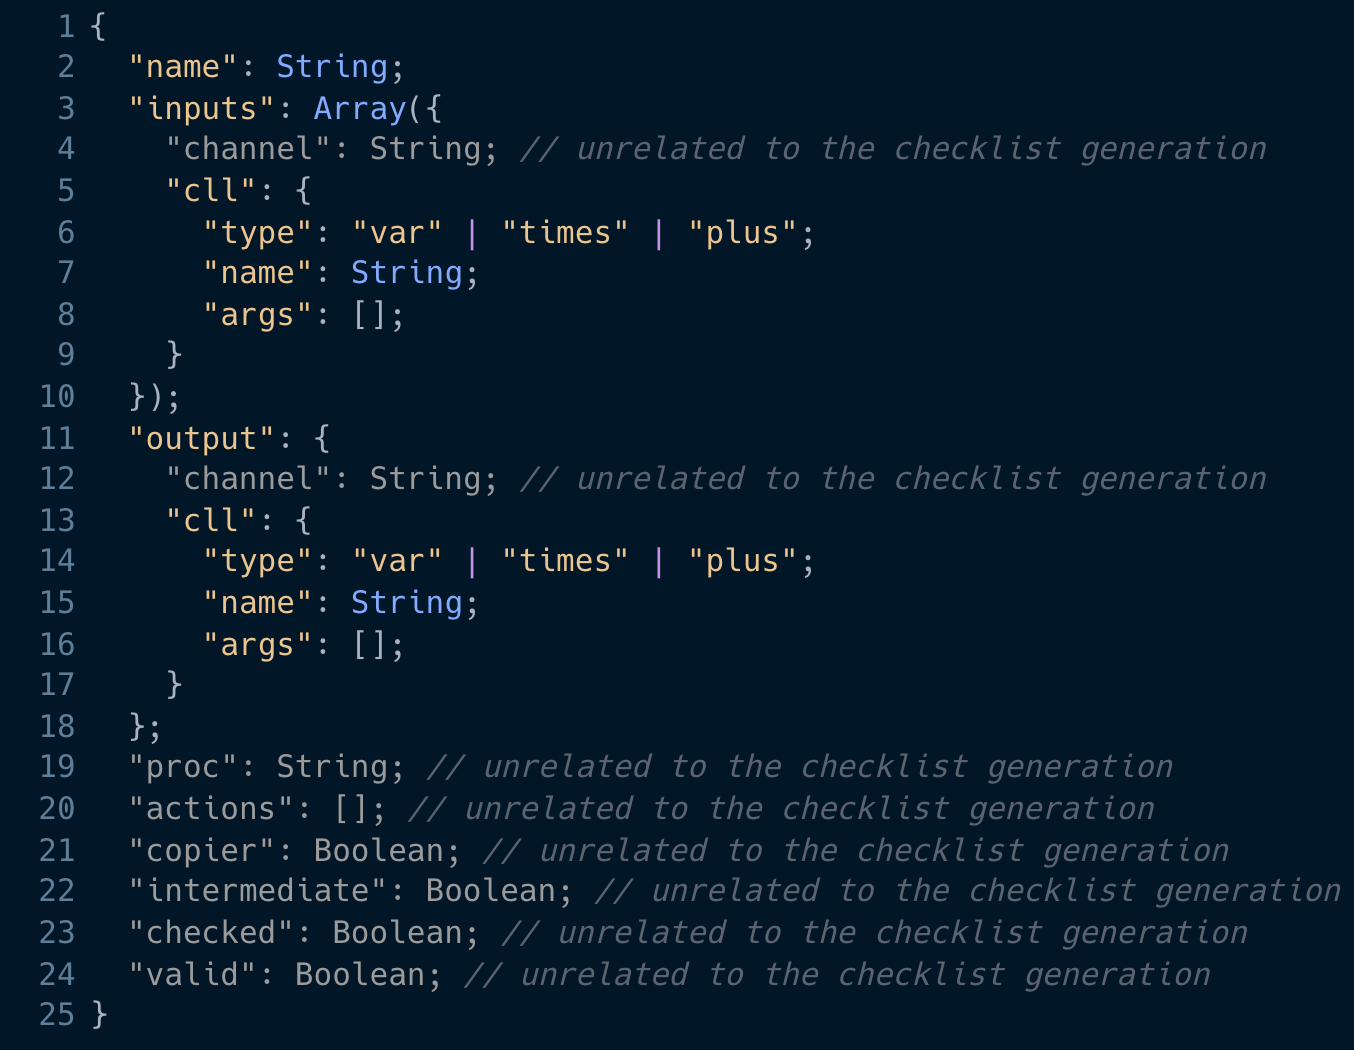
\includegraphics[width=0.85\textwidth]{overleaf/images/workflowfm_json.png}
%     \caption{WorkflowFM's Process JSON}
%     \label{appendix:fig:workflowfm_json}
% \end{figure}

\begin{figure}
    \centering
    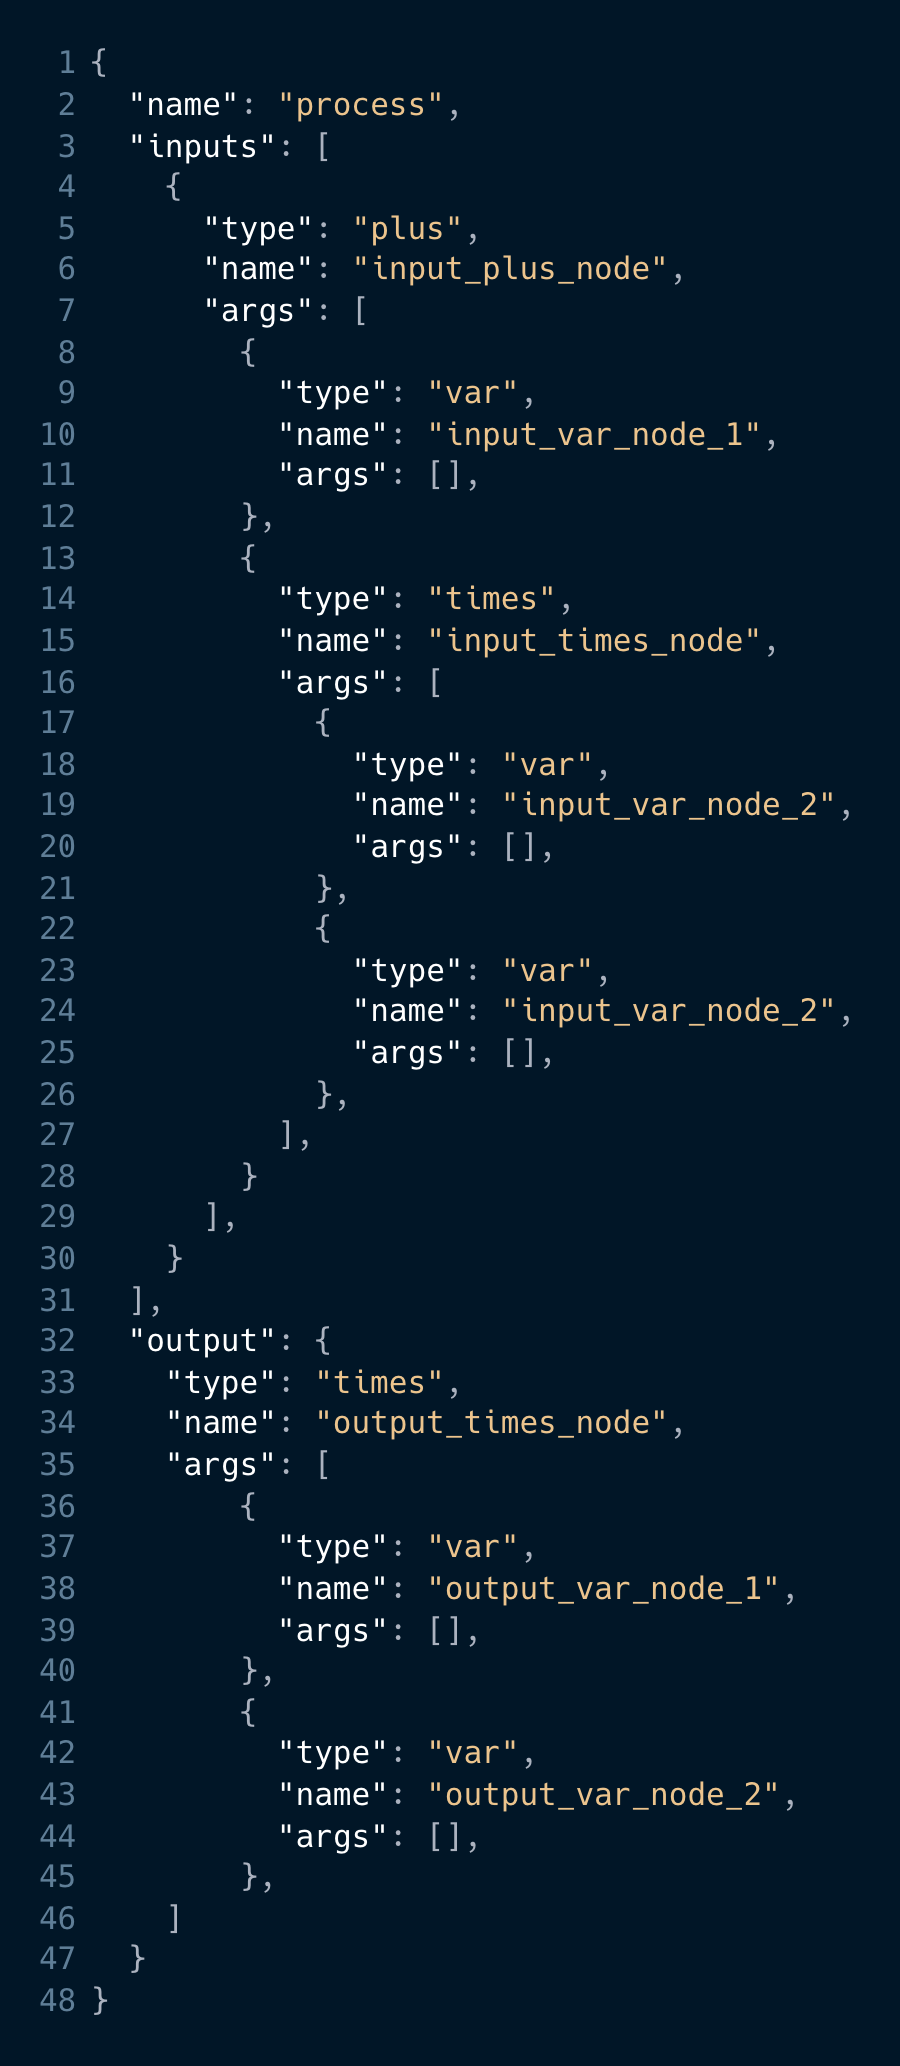
\includegraphics[width=0.65\textwidth]{overleaf/images/example_json.png}
    \caption{Figure \ref{fig:process_flows}'s JSON}
    \label{appendix:fig:example_json}
\end{figure}

\chapter{Design Appendix}
\begin{figure}[ht!]
    \centering
    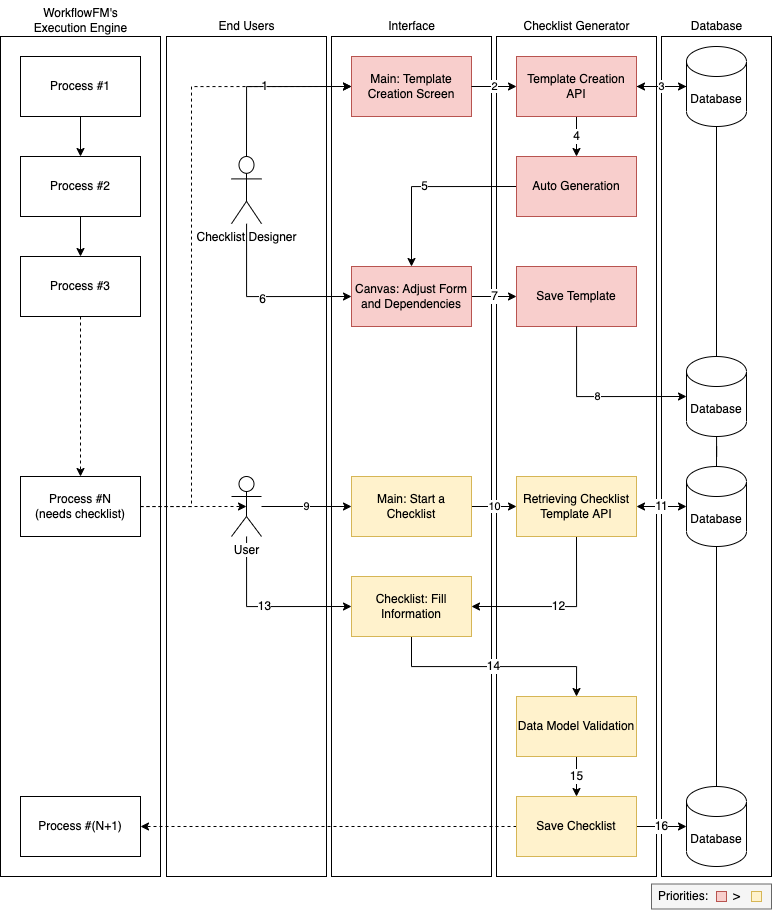
\includegraphics[width=\textwidth]{overleaf/images/overall_system_diagram_full.png}
    \caption{Detailed Overall System Diagram}
    \label{appendix:fig:overall_system_diagram}
\end{figure}


\begin{figure}[ht]
    \centering
    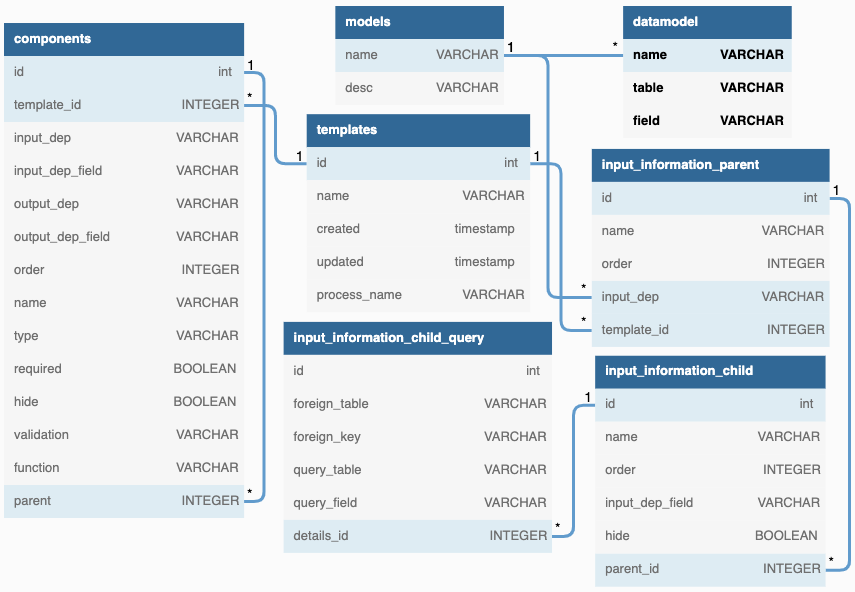
\includegraphics[width=\textwidth]{overleaf/images/checklist_db_design.png}
    \caption{Checklist Database Design}
    \label{fig:checklist_db_design}
\end{figure}

% \chapter{Sequence Diagrams}
% \label{appendix:sequence_diagrams}
% \begin{figure}[ht!]
%     \centering
%     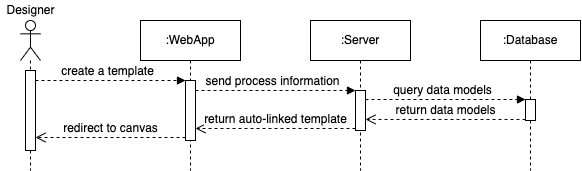
\includegraphics[width=\textwidth]{overleaf/images/create_template.png}
%     \caption{Sequence Diagram of Create Template Scenario}
%     \label{fig:create_template}
% \end{figure}


% \begin{figure}[ht!]
%     \centering
%     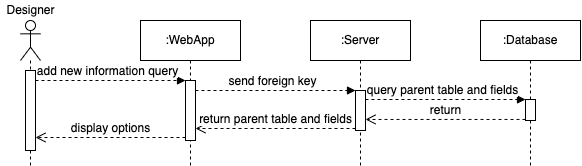
\includegraphics[width=\textwidth]{overleaf/images/add_new_information_query.png}
%     \caption{Sequence Diagram of Add New Information Query Scenario}
%     \label{fig:add_new_information_query}
% \end{figure}


% \begin{figure}[ht!]
%     \centering
%     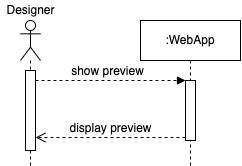
\includegraphics[width=0.4\textwidth]{overleaf/images/show_preview.png}
%     \caption{Sequence Diagram of Show Preview Scenario}
%     \label{fig:show_preview}
% \end{figure}


% \begin{figure}[ht!]
%     \centering
%     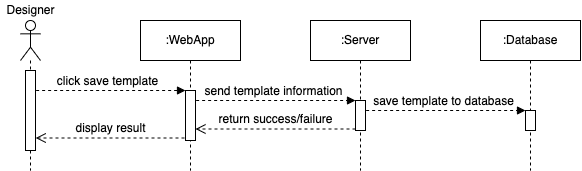
\includegraphics[width=\textwidth]{overleaf/images/save_template.png}
%     \caption{Sequence Diagram of Save Template Scenario}
%     \label{fig:save_template}
% \end{figure}


% \begin{figure}[ht!]
%     \centering
%     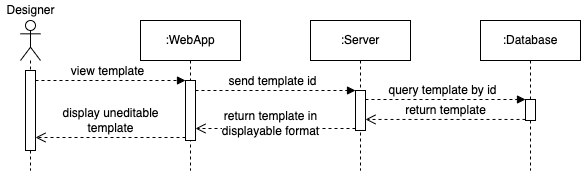
\includegraphics[width=\textwidth]{overleaf/images/view_template.png}
%     \caption{Sequence Diagram of View Template Scenario}
%     \label{fig:view_template}
% \end{figure}



\chapter{Auto Generation Psudocode}
\label{appendix:auto_gen_psudo}
\begin{figure}[ht!]
    \centering
    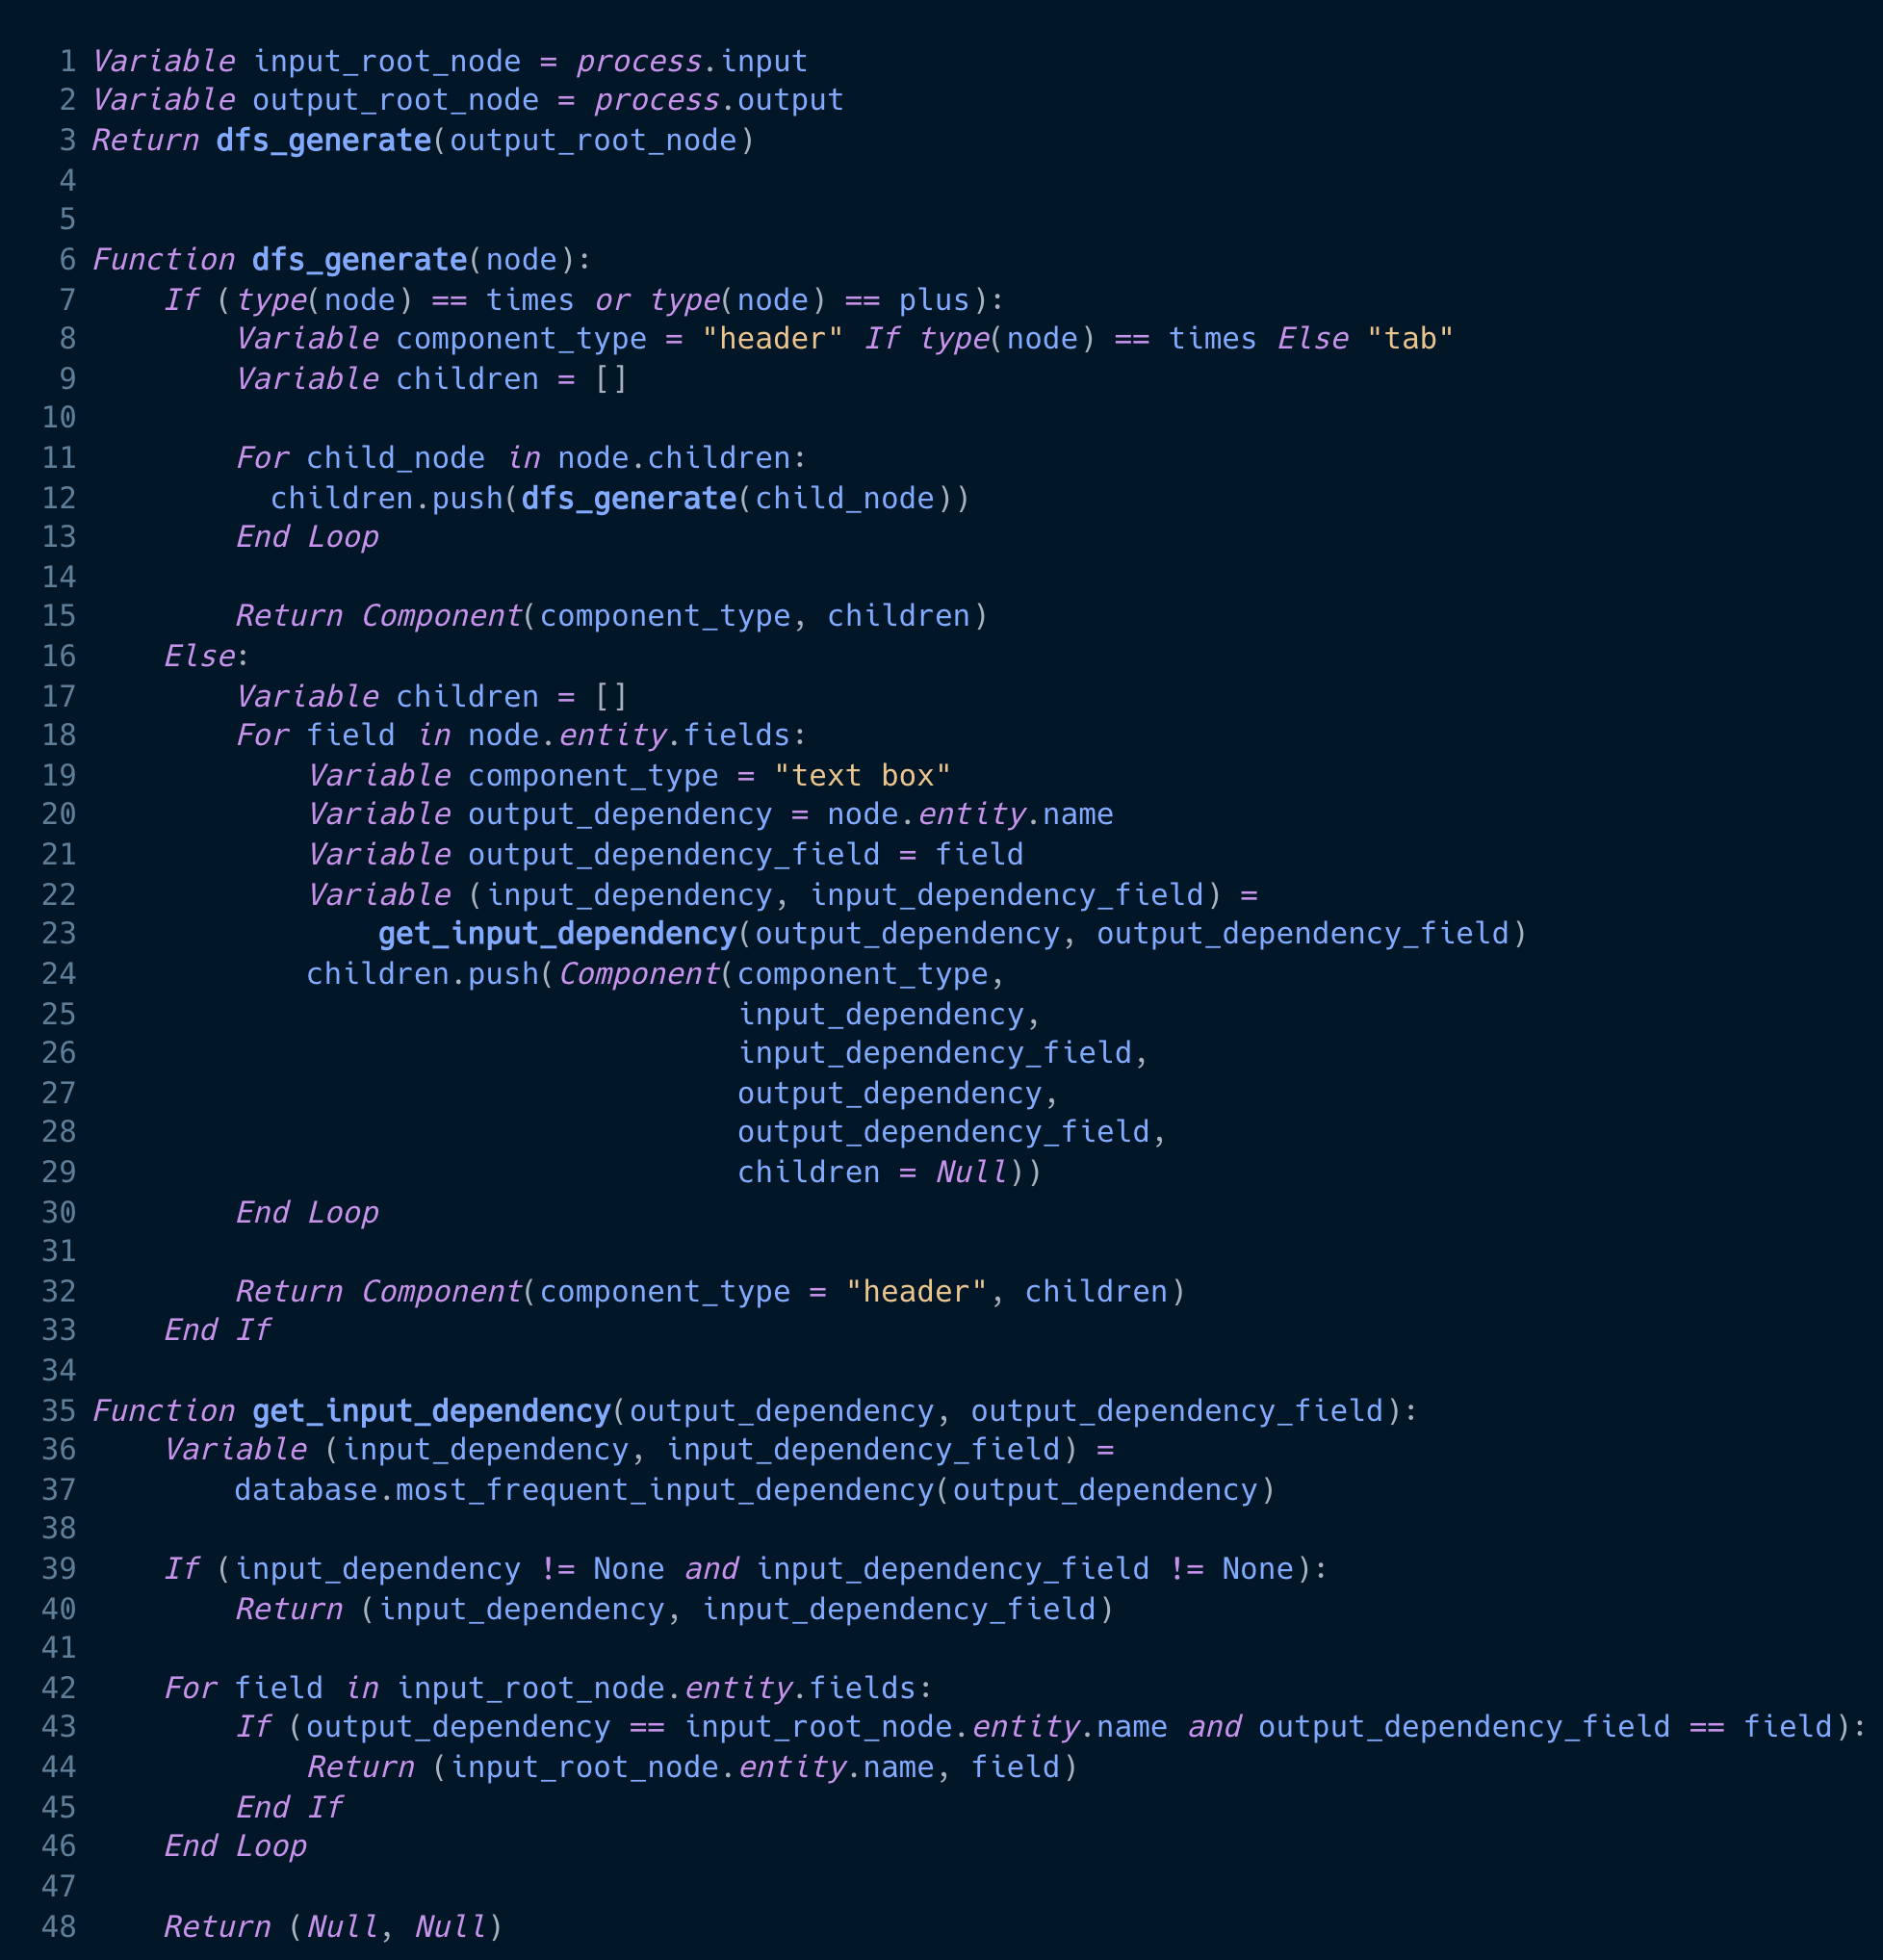
\includegraphics[width=\textwidth]{overleaf/images/auto_gen_psudo.png}
    \caption{Auto Generation's Psudocode}
    \label{fig:auto_gen_psudo}
\end{figure}




\chapter{Testing Examples}
\label{appendix:testing}

\begin{figure}
    \centering
    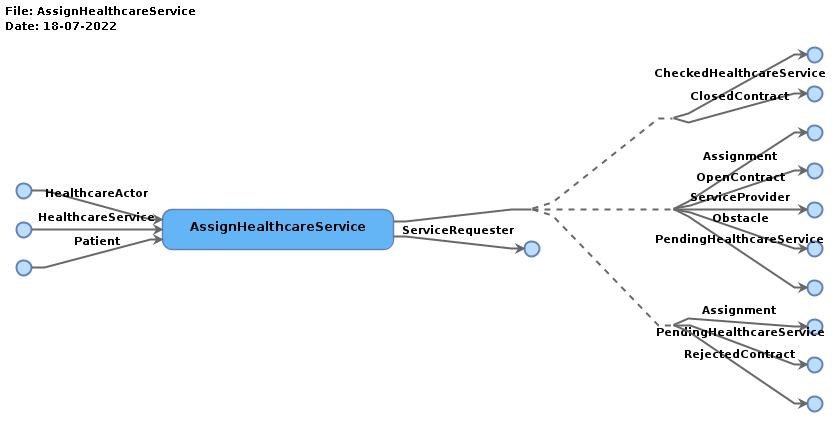
\includegraphics[width=\textwidth]{overleaf/images/testing/AssignHealthcareService.png}
    \caption{Assign Healthcare Service}
    \label{appendix:fig:AssignHealthcareService}
\end{figure}

\begin{figure}
    \centering
    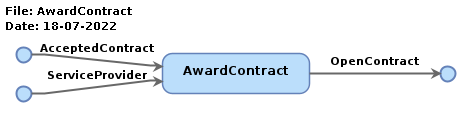
\includegraphics[width=\textwidth]{frontend/public/images/AwardContract.png}
    \caption{Award Contract}
    \label{appendix:fig:AwardContract}
\end{figure}

\begin{figure}
    \centering
    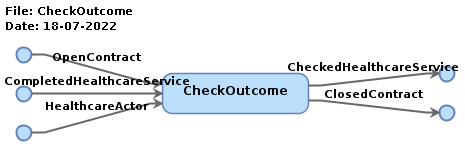
\includegraphics[width=\textwidth]{overleaf/images/testing/CheckOutcome.png}
    \caption{Check Outcome}
    \label{appendix:fig:CheckOutcome}
\end{figure}

\begin{figure}
    \centering
    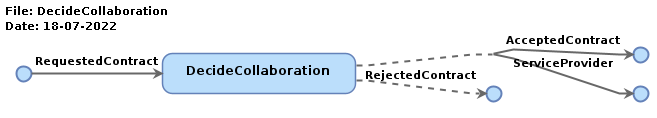
\includegraphics[width=\textwidth]{overleaf/images/testing/DecideCollaboration.png}
    \caption{Decide Collaboration}
    \label{appendix:fig:DecideCollaboration}
\end{figure}

\begin{figure}
    \centering
    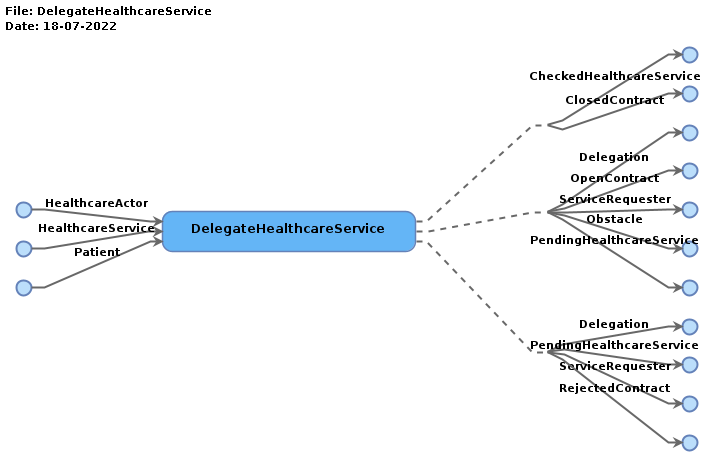
\includegraphics[width=\textwidth]{overleaf/images/testing/DelegateHealthcareService.png}
    \caption{Delegate Healthcare Service}
    \label{appendix:fig:DelegateHealthcareService}
\end{figure}

\begin{figure}
    \centering
    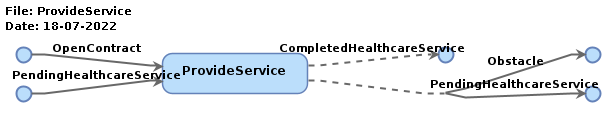
\includegraphics[width=\textwidth]{overleaf/images/testing/ProvideService.png}
    \caption{Provide Service}
    \label{appendix:fig:ProvideService}
\end{figure}

\begin{figure}
    \centering
    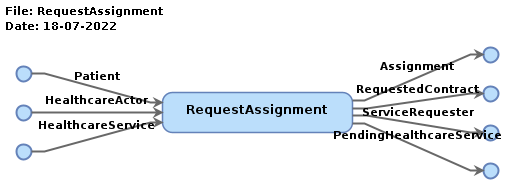
\includegraphics[width=\textwidth]{overleaf/images/testing/RequestAssignment.png}
    \caption{Request Assignment}
    \label{appendix:fig:RequestAssignment}
\end{figure}

\begin{figure}
    \centering
    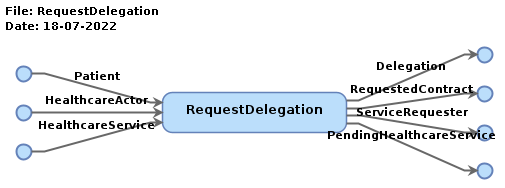
\includegraphics[width=\textwidth]{overleaf/images/testing/RequestDelegation.png}
    \caption{Request Delegation}
    \label{appendix:fig:RequestDelegation}
\end{figure}

\begin{figure}
    \centering
    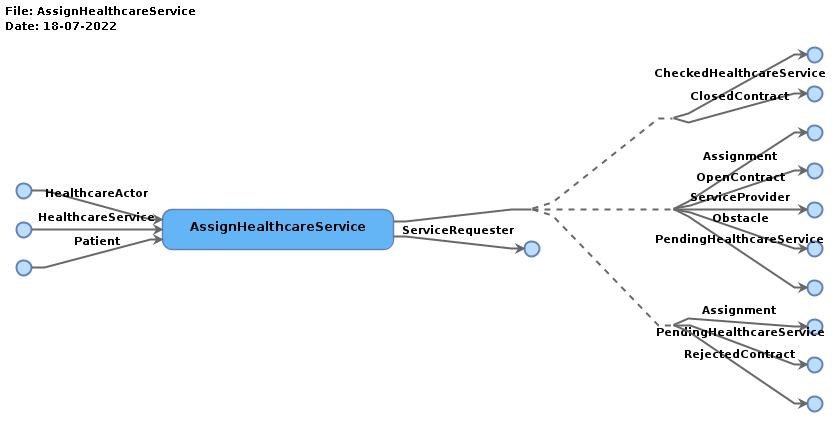
\includegraphics[width=\textwidth]{overleaf/images/testing/AssignHealthcareService.png}
    \caption{Assign Healthcare Service}
    \label{appendix:fig:AssignHealthcareService}
\end{figure}

\begin{figure}
    \centering
    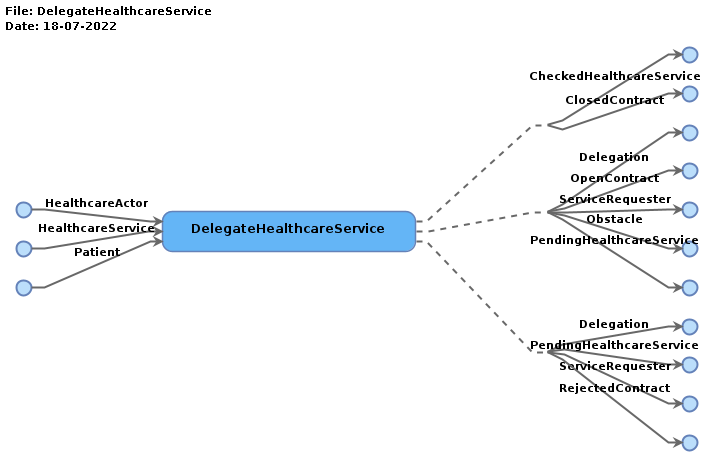
\includegraphics[width=\textwidth]{overleaf/images/testing/DelegateHealthcareService.png}
    \caption{Delegate Healthcare Service}
    \label{appendix:fig:DelegateHealthcareService}
\end{figure}


\chapter{Questionnaires}
\label{appendix:questionnaire}


\begin{table}[ht!]
    \centering
    \footnotesize
    \hspace*{\fill} \textbf{Disagree \qquad\quad\>\>\> Agree}
    \begin{tabular}{
      |p{\dimexpr.75\linewidth-2\tabcolsep-1.3333\arrayrulewidth}% column 1
      |p{\dimexpr.05\linewidth-2\tabcolsep-1.3333\arrayrulewidth}% column 2
      |p{\dimexpr.05\linewidth-2\tabcolsep-1.3333\arrayrulewidth}% column 2
      |p{\dimexpr.05\linewidth-2\tabcolsep-1.3333\arrayrulewidth}% column 2
      |p{\dimexpr.05\linewidth-2\tabcolsep-1.3333\arrayrulewidth}% column 2
      |p{\dimexpr.05\linewidth-2\tabcolsep-1.3333\arrayrulewidth}|% column 3
      }
      \hline
      \centering Questions & \centering 1 & \centering 2 & \centering 3 & \centering 4 & \centering\arraybackslash 5     \\ \hline
      1.) I was able to perform task 1 and task 2 successfully. &  & & &  & \\ \hline
      2.) I could easily query new input information for the fields. &  & & &  & \\ \hline
      3.) The form adjustment section was easy to use. &  & & &  & \\ \hline
      4.) I could easily add and adjust new form fields in the form adjustment section. &  & & &  & \\ \hline
      5.) I could easily link dependencies of each form field. &  & & &  & \\ \hline
      6.) The help tools (the query suggestion and the auto-generation) were easy to use. &  & & &  & \\ \hline
      7.) The help tools were helpful and made the whole process easier. &  & & &  & \\ \hline
    \end{tabular}
    \caption{First Functionality Questionnaire}
    \label{tab:1stfunctionality}
\end{table}


\begin{table}[ht!]
    \centering
    \footnotesize
    \hspace*{\fill} \textbf{Disagree \qquad\quad\>\>\> Agree}
    \begin{tabular}{
      |p{\dimexpr.75\linewidth-2\tabcolsep-1.3333\arrayrulewidth}% column 1
      |p{\dimexpr.05\linewidth-2\tabcolsep-1.3333\arrayrulewidth}% column 2
      |p{\dimexpr.05\linewidth-2\tabcolsep-1.3333\arrayrulewidth}% column 2
      |p{\dimexpr.05\linewidth-2\tabcolsep-1.3333\arrayrulewidth}% column 2
      |p{\dimexpr.05\linewidth-2\tabcolsep-1.3333\arrayrulewidth}% column 2
      |p{\dimexpr.05\linewidth-2\tabcolsep-1.3333\arrayrulewidth}|% column 3
      }
      \hline
      \centering Questions & \centering 1 & \centering 2 & \centering 3 & \centering 4 & \centering\arraybackslash 5     \\ \hline
      1.) I had no problem performing task 3 without any instructions. &  & & &  & \\ \hline
      2.) I could easily query new fields in the information input. &  & & &  & \\ \hline
      3.) Adjusting the form to the requirement was troublesome in this task. &  & & &  & \\ \hline
      4.) I found the help tools (query suggestion and auto-generation) provided in the system helpful and helped me to perform this task. &  & & &  & \\ \hline
    \end{tabular}
    \caption{Second Functionality Questionnaire}
    \label{tab:2ndfunctionality}
\end{table}

\begin{table}[ht!]
    \centering
    \footnotesize
    \hspace*{\fill} \textbf{Disagree \qquad\quad\>\>\> Agree}
    \begin{tabular}{
      |p{\dimexpr.75\linewidth-2\tabcolsep-1.3333\arrayrulewidth}% column 1
      |p{\dimexpr.05\linewidth-2\tabcolsep-1.3333\arrayrulewidth}% column 2
      |p{\dimexpr.05\linewidth-2\tabcolsep-1.3333\arrayrulewidth}% column 2
      |p{\dimexpr.05\linewidth-2\tabcolsep-1.3333\arrayrulewidth}% column 2
      |p{\dimexpr.05\linewidth-2\tabcolsep-1.3333\arrayrulewidth}% column 2
      |p{\dimexpr.05\linewidth-2\tabcolsep-1.3333\arrayrulewidth}|% column 3
      }
      \hline
      \centering Questions & \centering 1 & \centering 2 & \centering 3 & \centering 4 & \centering\arraybackslash 5     \\ \hline
      1.) I think that I would like to use this system frequently. &  & & &  & \\ \hline
      2.) I found the system unnecessarily complex. &  & & &  & \\ \hline
      3.) I thought the system was easy to use. &  & & &  & \\ \hline
      4.) I think that I would need the support of a technical person to be able to use this system. &  & & &  & \\ \hline
      5.) I found the various functions in this system were well integrated. &  & & &  & \\ \hline
      6.) I thought there was too much inconsistency in this system. &  & & &  & \\ \hline
      7.) I would imagine that most people would learn to use this system very quickly. &  & & &  & \\ \hline
      8.) I found the system very cumbersome to use. &  & & &  & \\ \hline
      9.) I felt very confident using the system. &  & & &  & \\ \hline
      10.) I needed to learn a lot of things before I could get going with this system. &  & & &  & \\ \hline
      11.) After learning through the instructions, I would be able to create a checklist template by myself. &  & & &  & \\ \hline
      12.) The help tools (the query suggestion and the auto-generation) made it easier to create a template. &  & & &  & \\ \hline
    \end{tabular}
    \caption{Usability Questionnaire}
    \label{tab:usability}
\end{table}

\chapter{Questionnaire Scores}
\label{appendix:questionnaire_scores}

\begin{table}[ht!]
    \centering
    \footnotesize
    \begin{tabular}{
      |p{\dimexpr.2\linewidth-2\tabcolsep-1.3333\arrayrulewidth}% column 1
      |p{\dimexpr.15\linewidth-2\tabcolsep-1.3333\arrayrulewidth}% column 2
      |p{\dimexpr.15\linewidth-2\tabcolsep-1.3333\arrayrulewidth}|% column 3
      }
      \hline
      \centering Question & \centering Mean & \centering\arraybackslash SD    \\ \hline
      \hfil Q1 & \hfil 3.54 & \hfil 0.66 \\ \hline
      \hfil Q2 & \hfil 2.85 & \hfil 1.07 \\ \hline
      \hfil Q3 & \hfil 3.62 & \hfil 0.87 \\ \hline
      \hfil Q4 & \hfil 2.31 & \hfil 1.32 \\ \hline
      \hfil Q5 & \hfil 4.15 & \hfil 0.55 \\ \hline
      \hfil Q6 & \hfil 2.00 & \hfil 1.08 \\ \hline
      \hfil Q7 & \hfil 3.38 & \hfil 1.12 \\ \hline
      \hfil Q8 & \hfil 2.54 & \hfil 0.88 \\ \hline
      \hfil Q9 & \hfil 3.38 & \hfil 0.87 \\ \hline
      \hfil Q10 & \hfil 3.15 & \hfil 0.90 \\ \hline
      \hfil \textbf{SUS Score} & \hfil \textbf{63.08} & \hfil \textbf{15.00} \\ \hline
    \end{tabular}
    \caption{Usability Scores}
    \label{tab:sus_score}
\end{table}



% \chapter{Participants' information sheet}
% \label{pis}
% 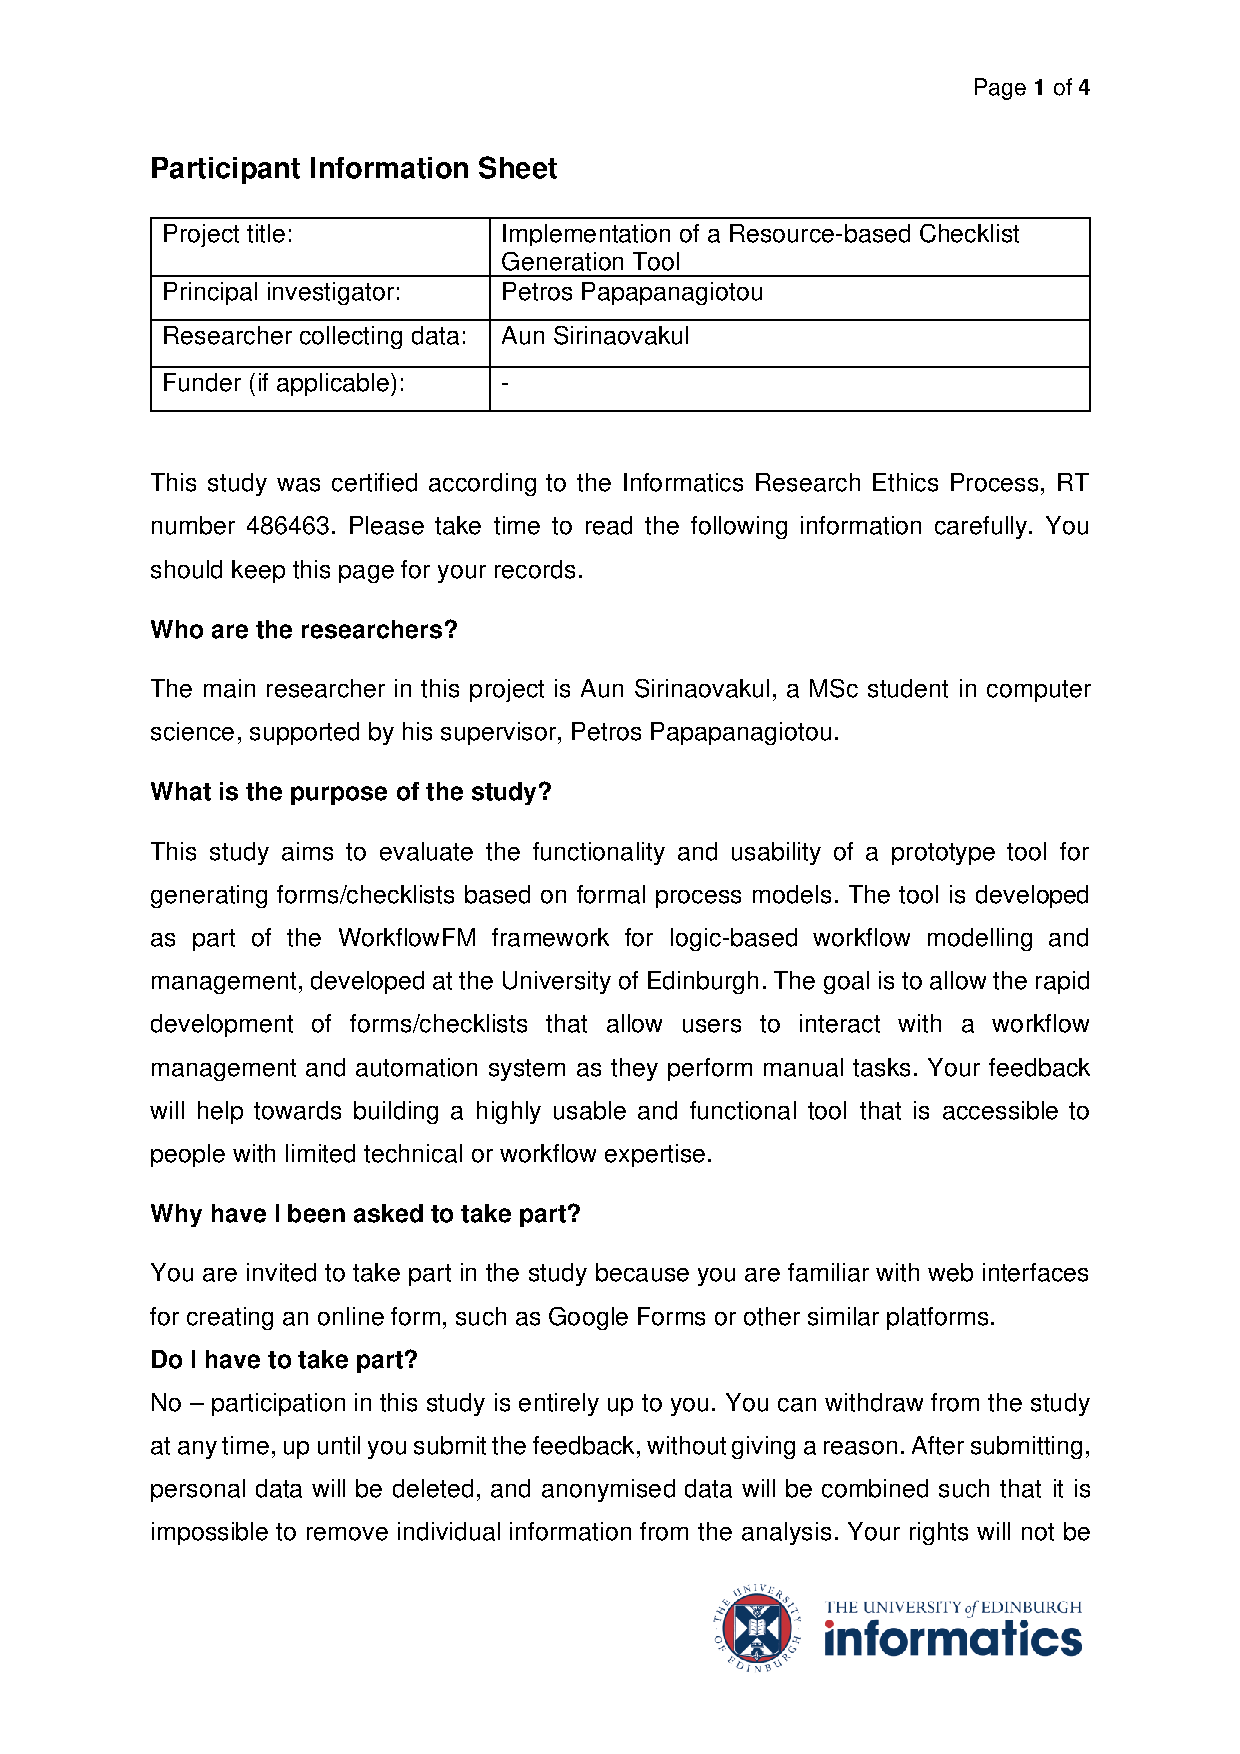
\includepdf[pages=-]{./pdf/Participant Information Sheet .pdf}

% \chapter{Participants' consent form}
% \label{pcf}
% 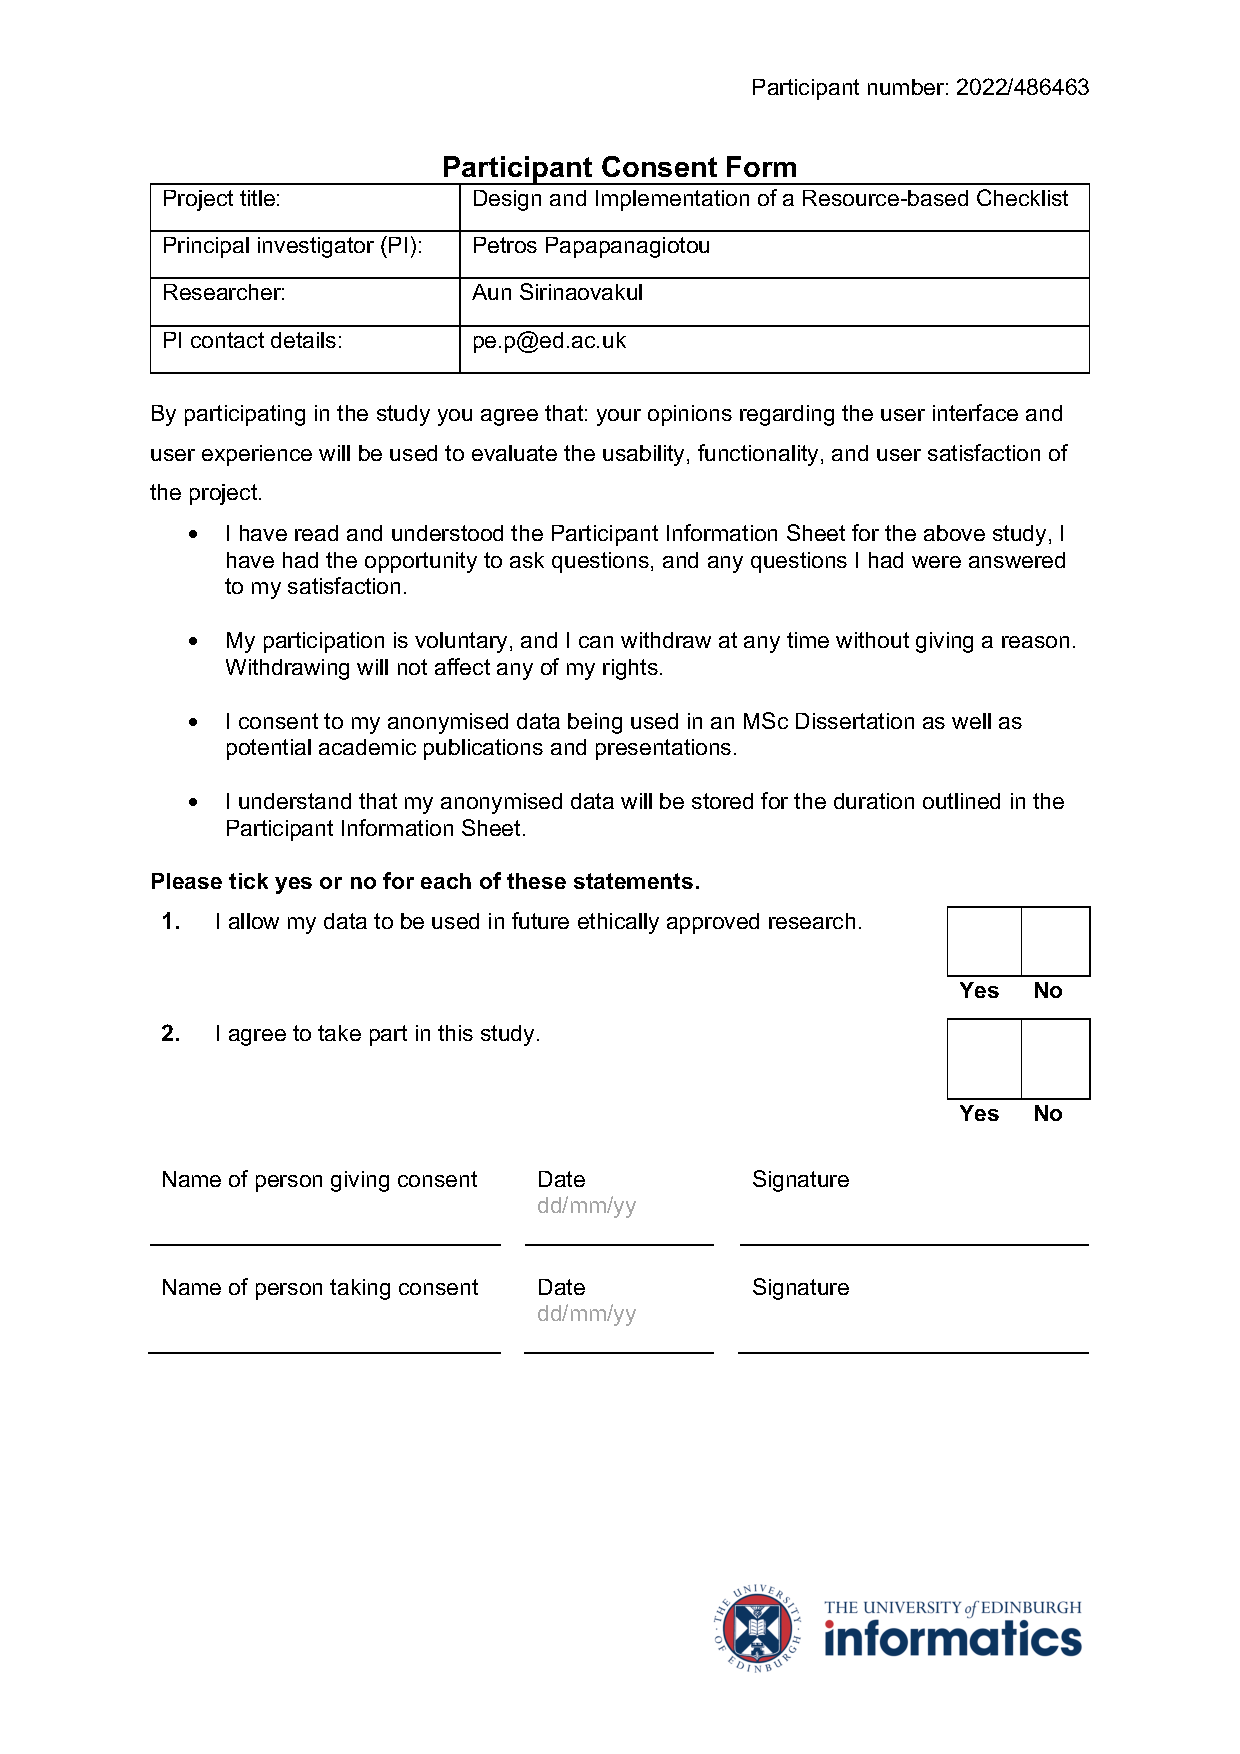
\includepdf[pages=-]{./pdf/Consent Form.pdf}

% \chapter{User Evaluation Document}
% \label{appendeix_evaluation}
% 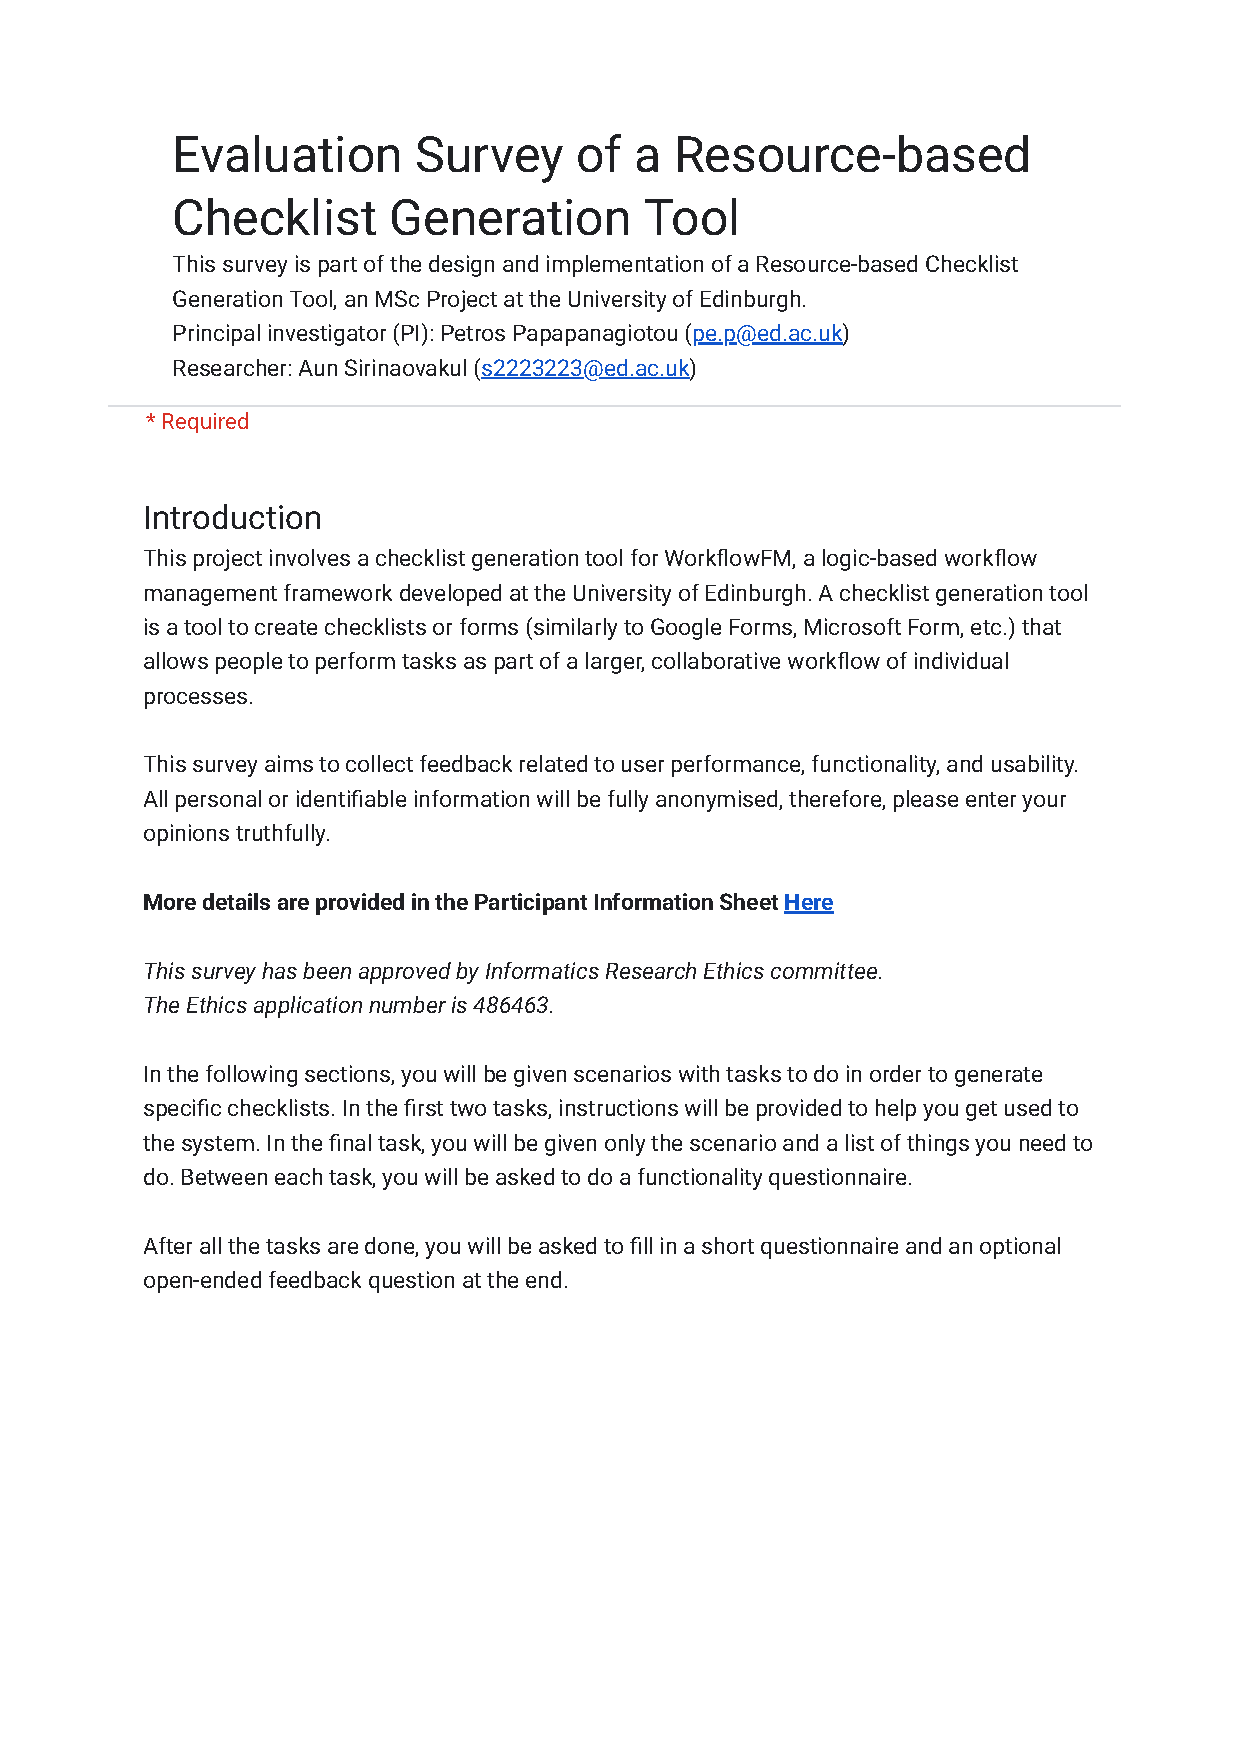
\includepdf[pages=-]{./pdf/Evaluation Survey of a Resource-based Checklist Generation Tool - Google Forms.pdf}
